\documentclass{article}
\title{Testing How Dust Affects the PMD Camera's Depth Accuracy}
\date{July\\3\\2019}
\author{Aaron Jencks\\Electronics Technology Technician Intern, JET Engineering}

\usepackage{pgfplots}

\usepackage{graphicx}
\usepackage{media9}

\usepackage{listings}

\usepackage{hyperref}
\hypersetup{
	colorlinks=true,
	linkcolor=blue,
	filecolor=magenta,
	urlcolor=cyan,
}

\begin{document}
	\maketitle
	\newpage
	
	\tableofcontents
	
	\newpage
	
	\section{Summary}
		This experiment was performed to determine if dusty environments can effect the performance of the PMD camera's depth accuracy, dust will be dropped in front of the camera, followed by ~30-45 seconds of depth data collection, if the depth values changed significantly during that time, then we should conclude that dust affects performance.
		
		\subsection{Hypothesis}
			I think that if we throw up dust in front of the camera and then continuously record depth data from it, for about 30 seconds, we should see the depth accuracy be sharply incorrect to start with, and then gradually return to normal as the dust settles.
		
	\section{Setup}
		\subsection{Materials}
			\begin{enumerate}
				\item PMD Camera (for ours we used a picoflex)
				\item The RoyaleSDK (make sure /python is added to PYTHONPATH environment variable)
				\item Dusty, dry dirt (to generate the dust from)
				\item A box large enough to fill the camera's field of view and to hold the bin of dirt at the same time
				\item A mount for the camera
				\item A ventilation fan
				\item A particle ventilation mask
			\end{enumerate}
		
		\newpage
		
		\subsection{Our Setup}
			Explain how to setup your experiment here, below is an example of how to include an image.
			
			\begin{figure}[h]
				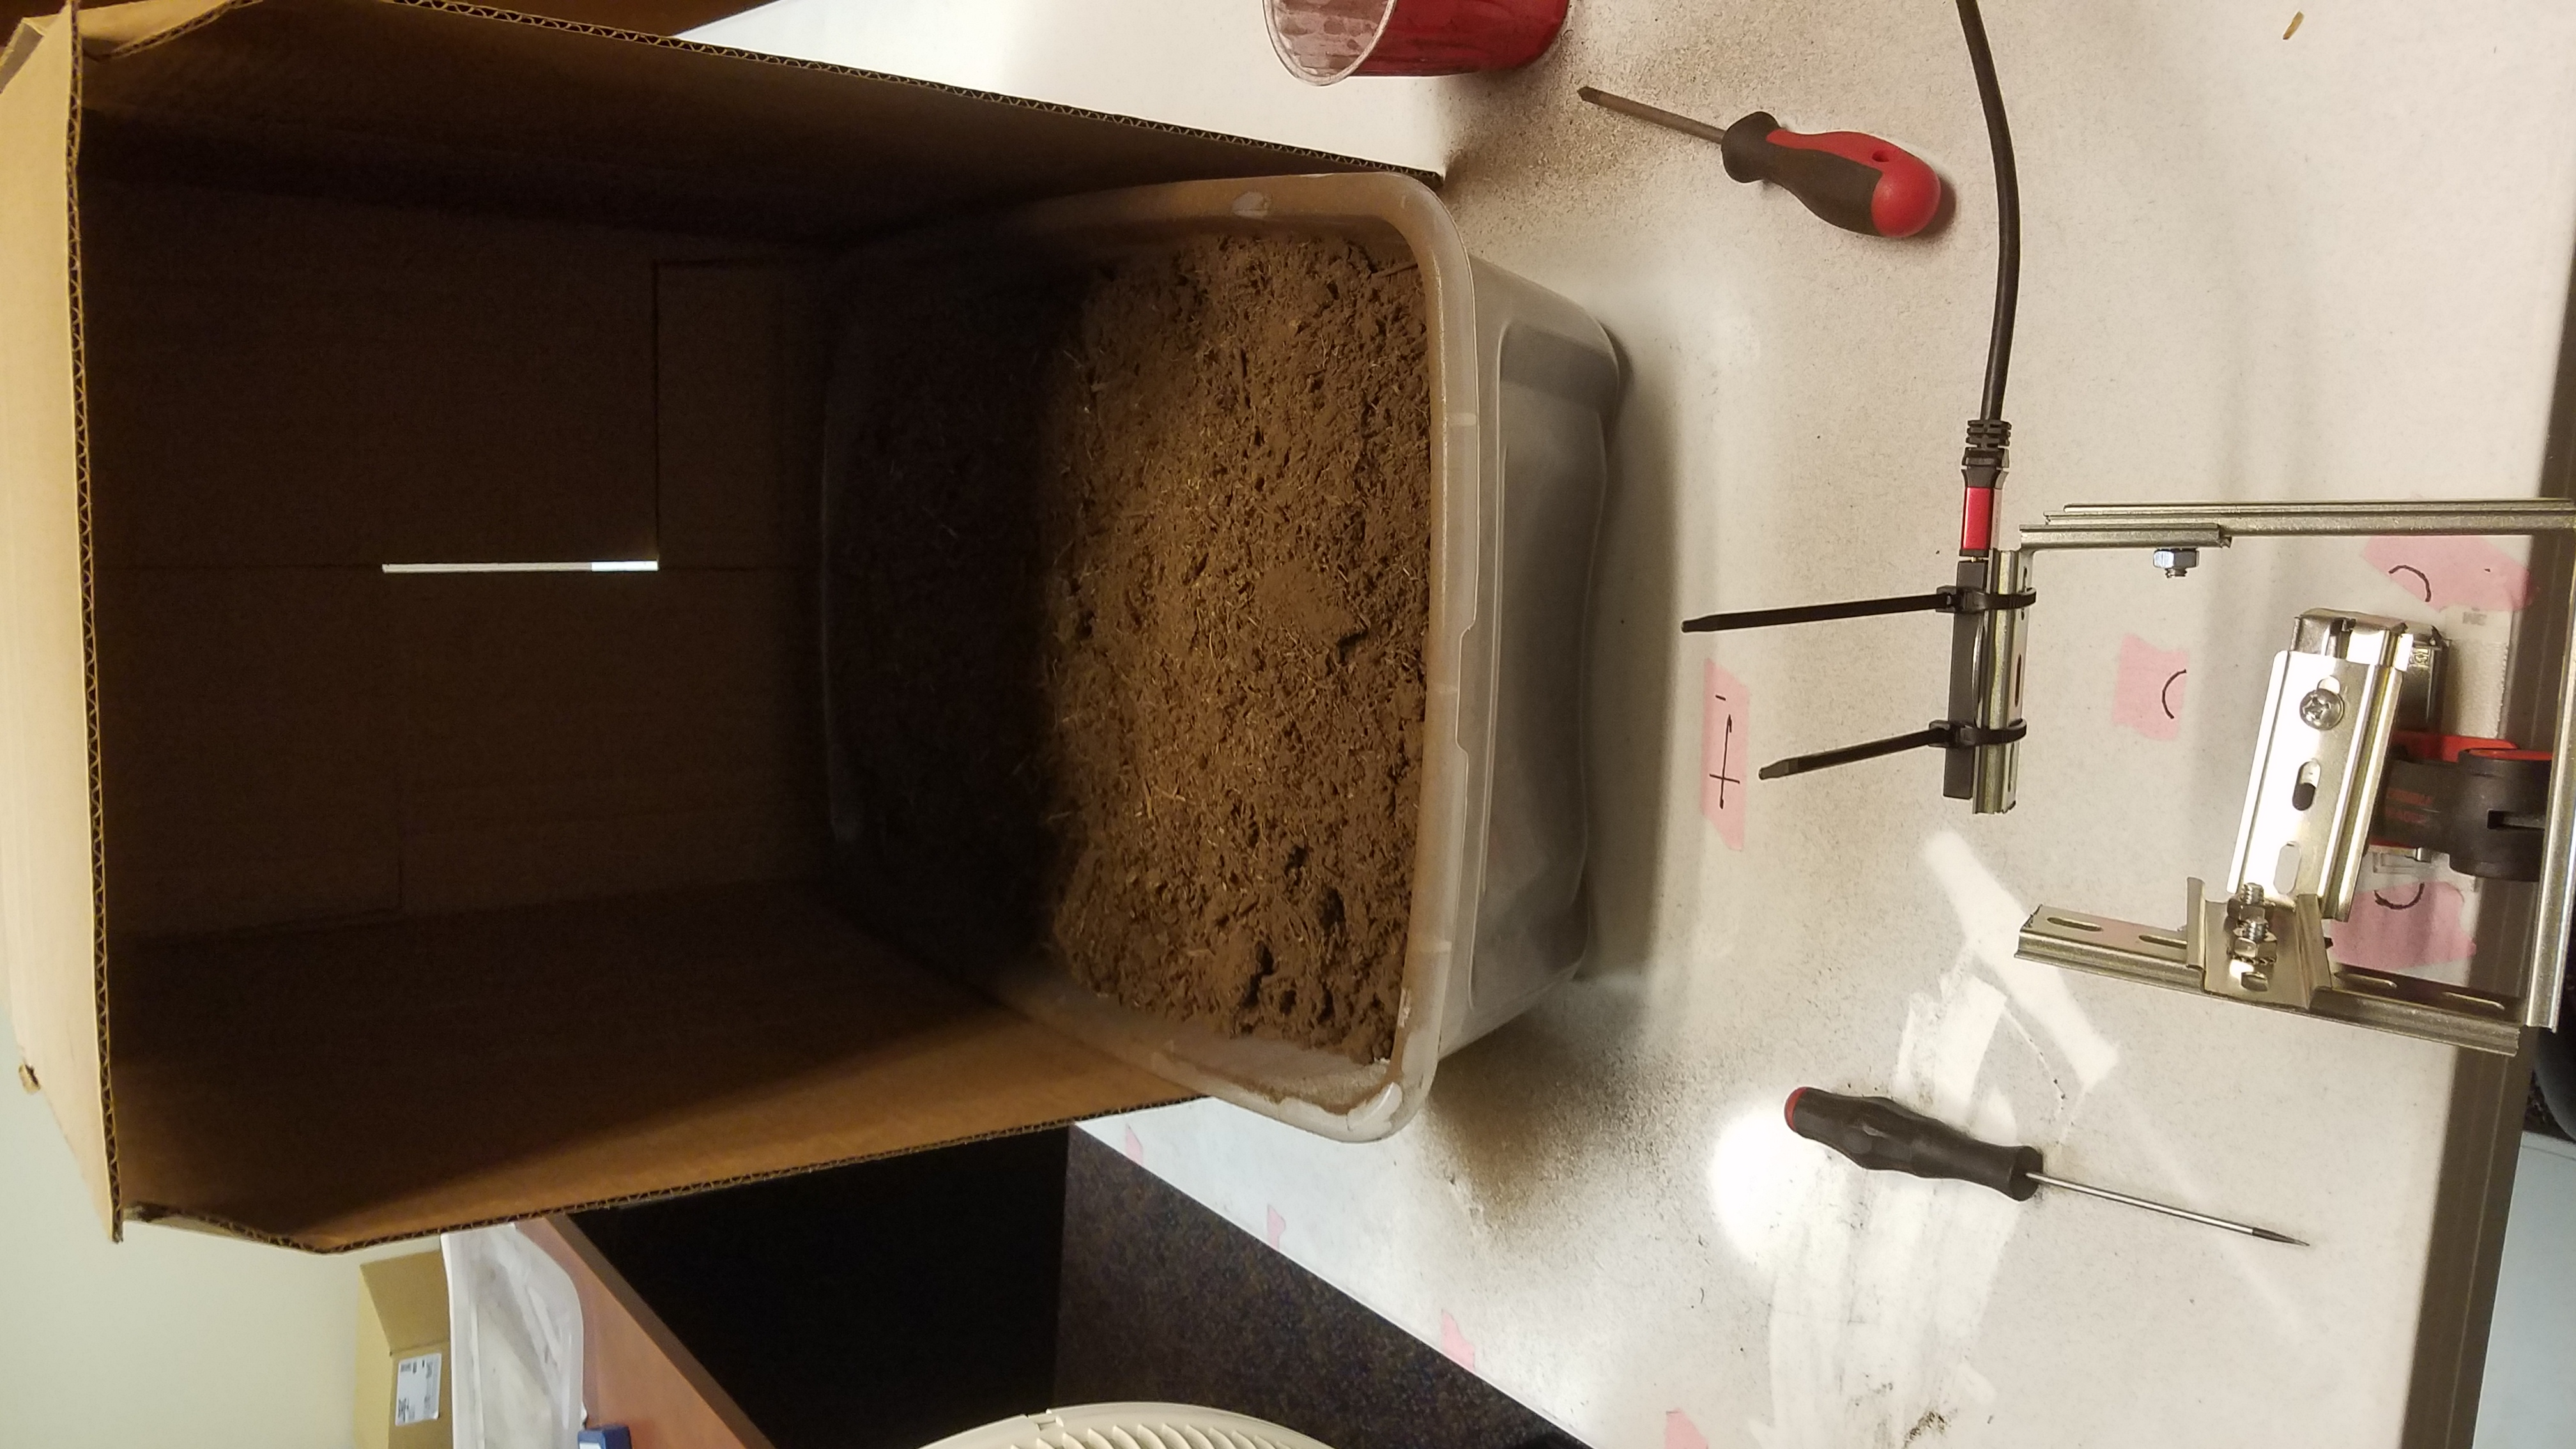
\includegraphics[angle=270, origin=c, height=8cm]{./images/our_setup.jpg}
				\centering
				\caption{Our setup}
				\label{fig:setup}
			\end{figure}
			
	\section{Process}
		For this experiment, I used an automated data collection program, to help me collect the depth data quickly and accurately, this is described below.
		
		\newpage
		
		\subsection{The Code}
			I used python for the language, because of its ease of use, and since I have a majority of the code written for this already.
			You can find the code in the pmd\_dust\_test directory of the repo.  It's pretyy simple to run, there are 2 settings that you can control before execution
			\begin{itemize}
				\item duration
				\item roi
			\end{itemize}
			\paragraph{duration} This allows you to control how long the camera will capture for, default is 30 seconds
			\paragraph{roi} This allows you to control the region of interest that the camera will focus on during capture, only the data from this region will be collected and averaged.
			
			\subsubsection{Execution} The program asks you for a filename to save the data to while you are executing the test, it stores it in a tab-delimitted format, there is one line for each frame that was collected, each line is formatted as follows:
			
			\begin{lstlisting}
trial# | elapsed time in sec | avg depth | std dev
			\end{lstlisting}
			
		\subsection{Setup}
			As you can see in Figure \ref{fig:setup} place the camera on a mount, shown below is an example, see \ref{fig:mount}. Place the container with dirt inside of some sort of isolating chamber, such as a cardboard box, this keeps the dust in place longer so that the effect can be seen more easily and stops the dust from spreading around the room.  Point the camera into the box, run the royaleviewer and adjust the camera until you can see the back of the box and very little else, see Figure \ref{fig:viewer}.
			
			\begin{figure}[h]
				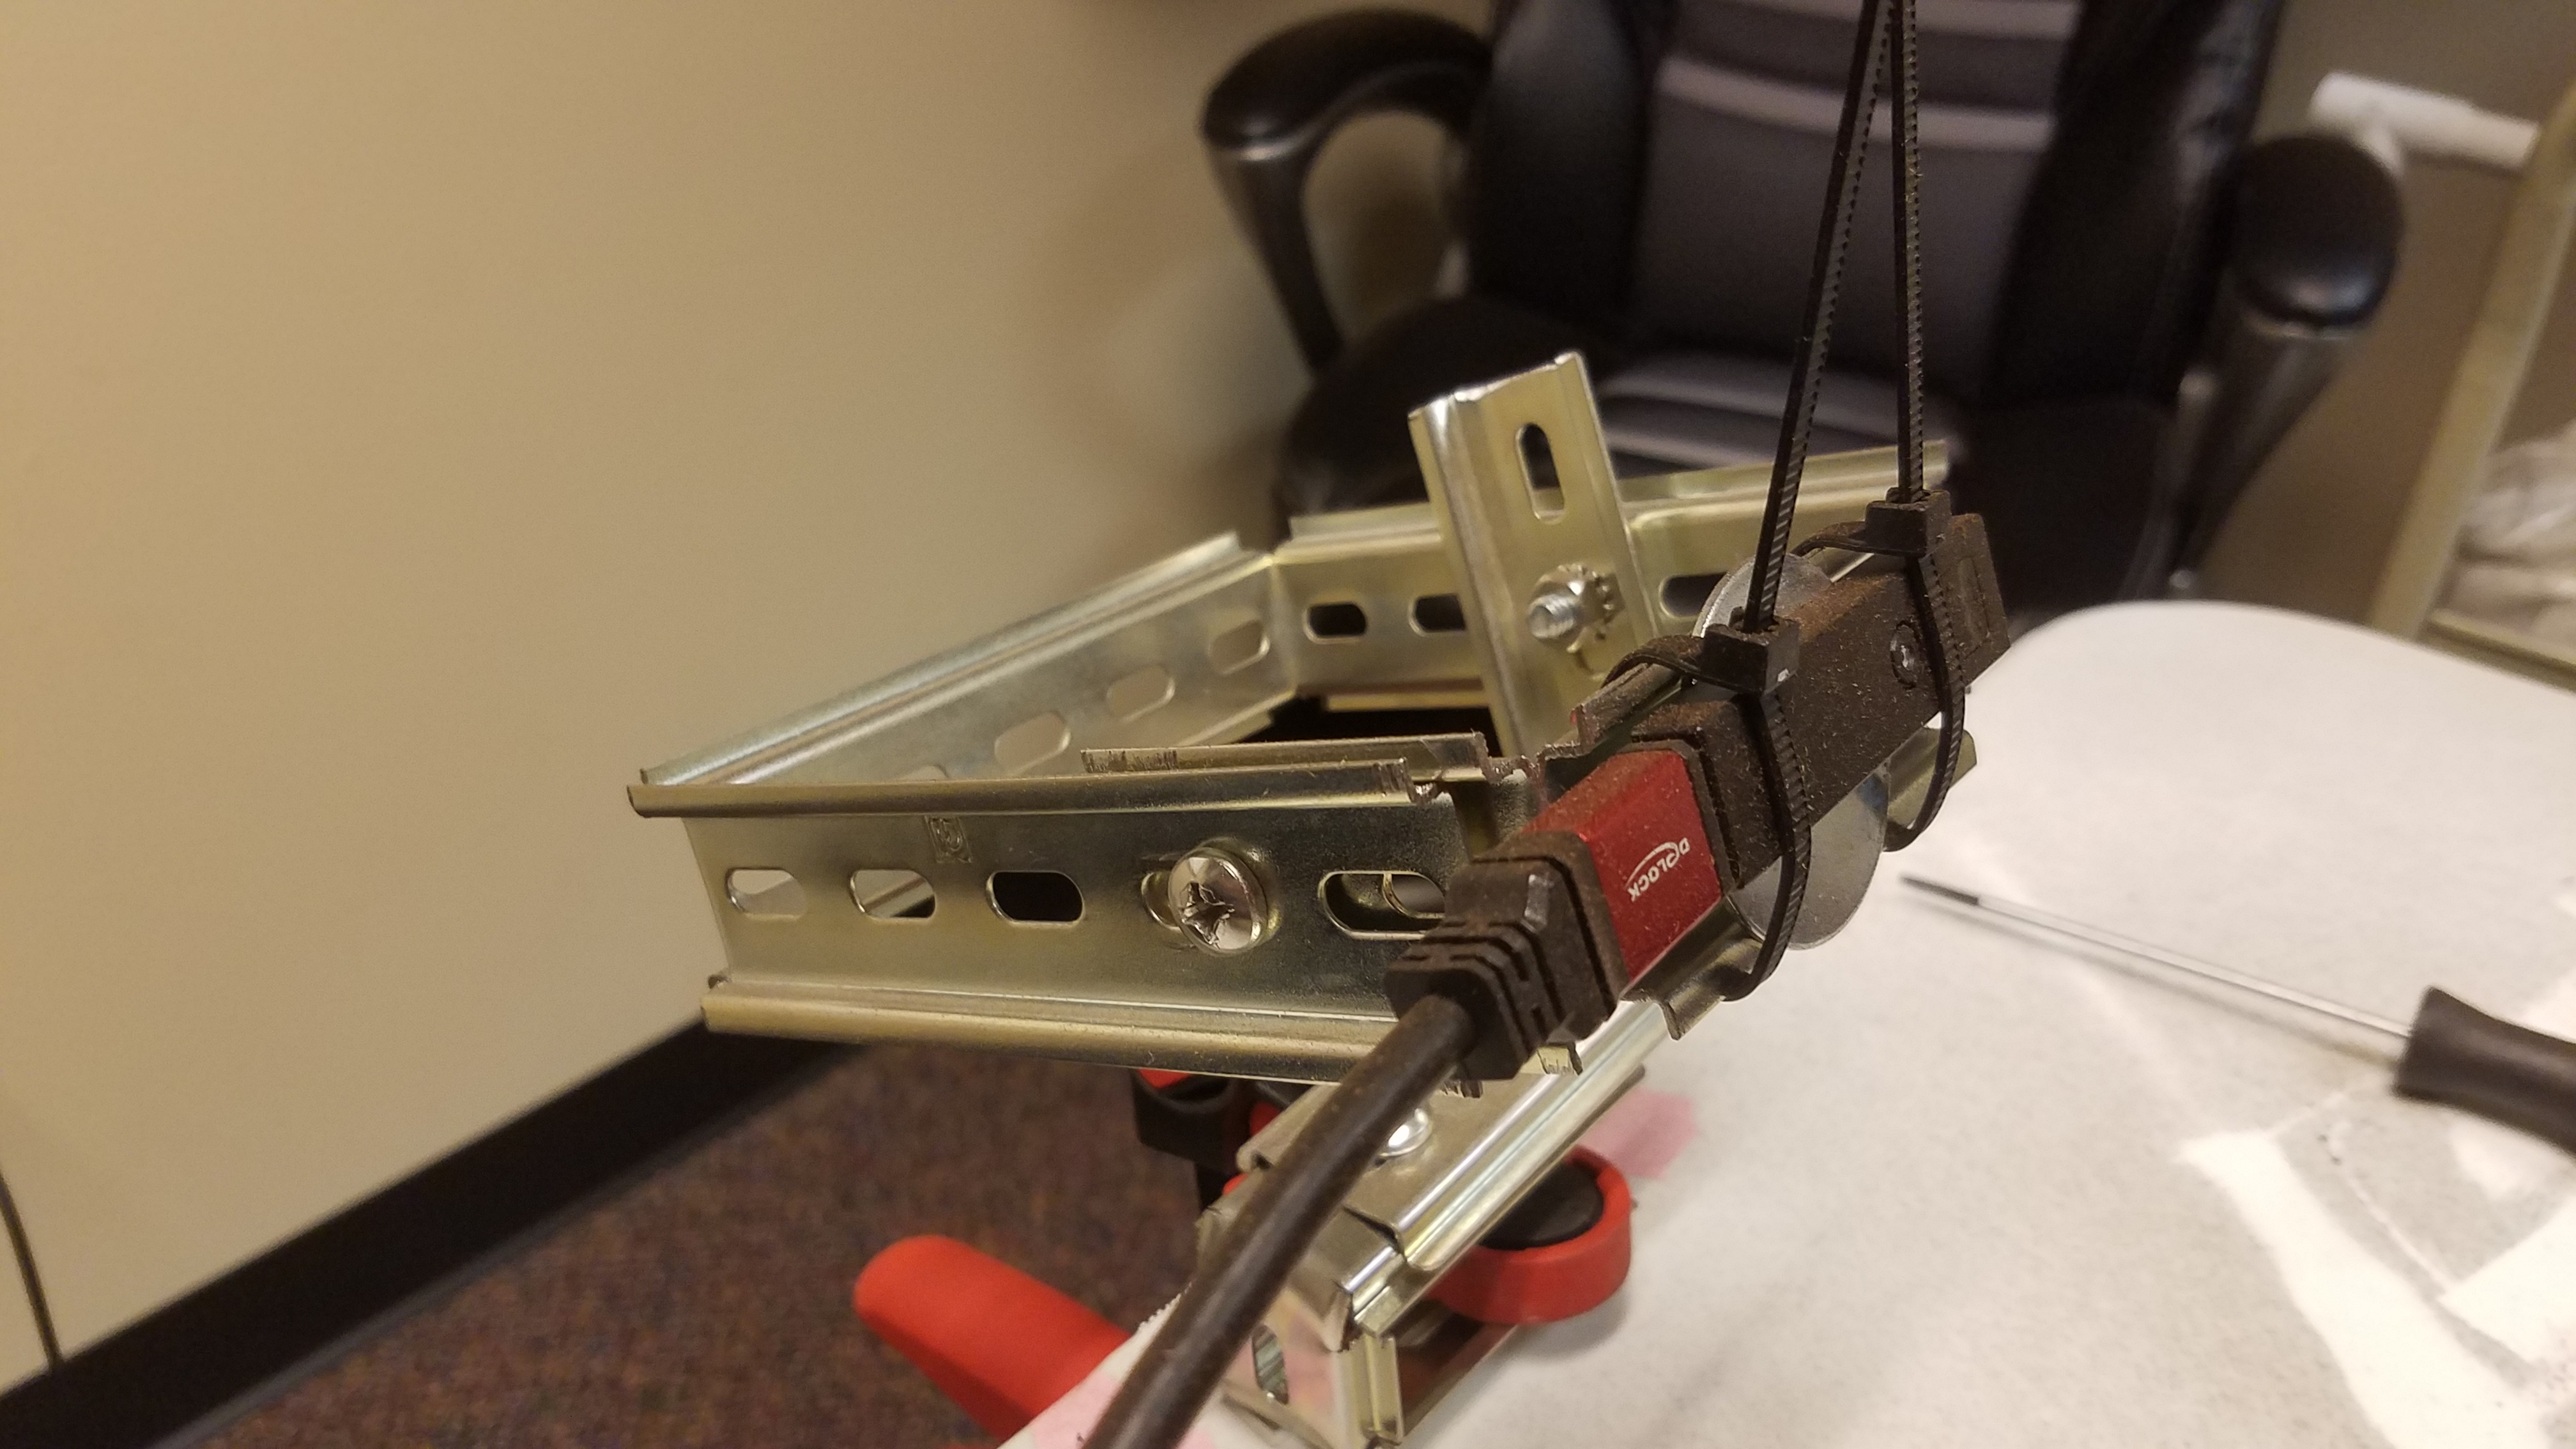
\includegraphics[width=8cm]{./images/mounting_system.jpg}
				\centering
				\caption{Example Mounting System}
				\label{fig:mount}
			\end{figure}
		
			\begin{figure}[h]
				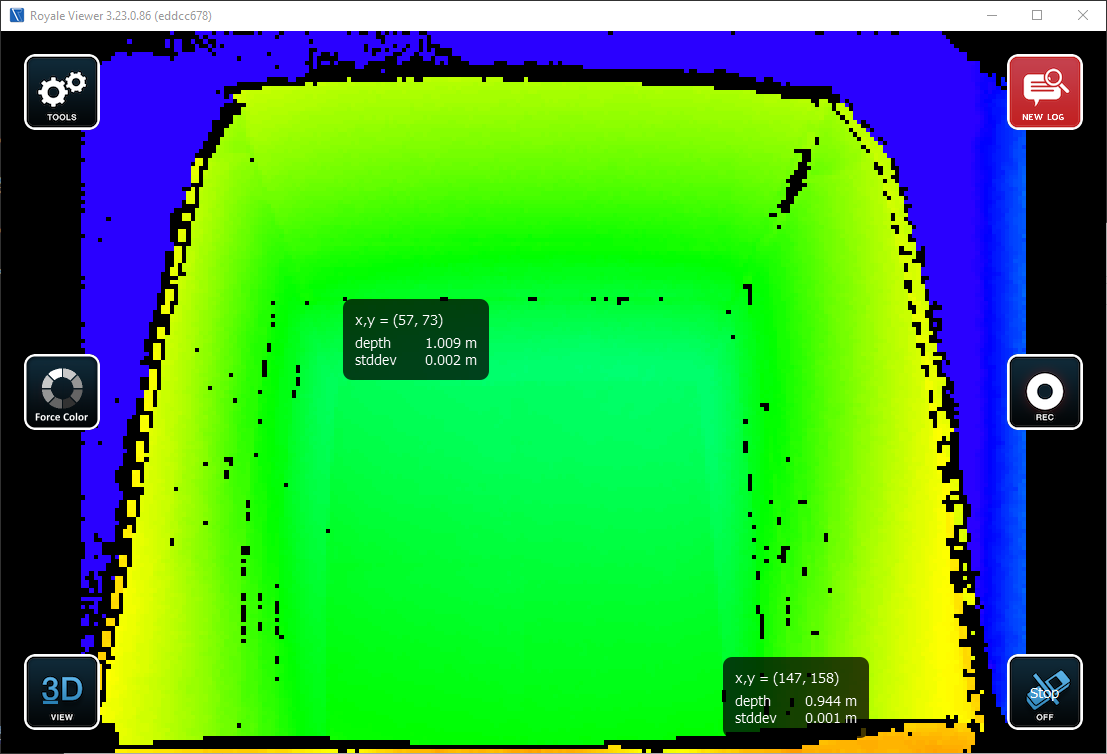
\includegraphics[width=8cm]{./images/royale_viewer_setup.png}
				\centering
				\caption{Finding the ROI using the RoyaleViewer}
				\label{fig:viewer}
			\end{figure}
		
			Once you've adjusted the camera to see the back of the box, then click near the top left corner and the lower right corner of the back of the box. This will bring up two windows that display the pixels of those corners, in the python script, modify the roi variable (see \ref{code:roi_variable}), to contain the data shown in your boxes.
			
			\label{code:roi_variable}
			\begin{lstlisting}[language=python]
roi = [68, 66, 163, 157]
			\end{lstlisting}
			
			\paragraph{Where} the values correspond to the layout below
			
			\begin{lstlisting}
upper left corner coordinate = (l, u)
lower right corner coordinate = (r, b)

roi = [l, u, r, b]
			\end{lstlisting}
		
			Next, start the program and let it run one trial with no dust in the air, we will use this as a baseline. Next you need to put on the particle mask and ensure the ventilation fan is off, disturb the dirt (and I mean really toss it around) to get some dust in the air inside of the box. Once the dust is really flying, click on the console and press any key to start recording the camera for 30 seconds. Repeat tossing the dirt and recording until the desired number of trials have been completed.
		
	\newpage
		
	\section{Results}
		After completing the desired number of trials, here is the average depth data for each trial, first one is the baseline with no dust.
		
		\begin{figure}[h]
			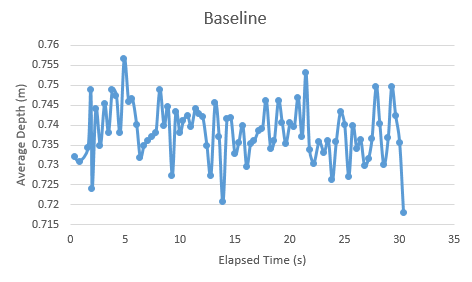
\includegraphics[width=8cm]{./images/results_baseline.png}
			\centering
			\caption{Baseline Results (no dust)}
			\label{fig:baseline}
		\end{figure}
	
		\begin{figure}[h]
			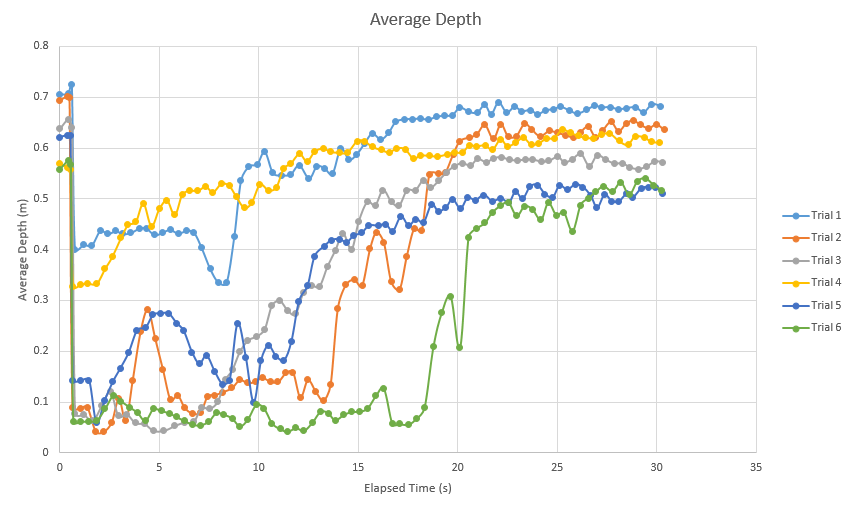
\includegraphics[width=8cm]{./images/results_depth.png}
			\centering
			\caption{Depth Results (with dust)}
			\label{fig:depth}
		\end{figure}
		
		\subsection{Discussion}
			As you can see, just as I suspected, when the dust is still in the box (actively settling), the depth accuracy plummets and slowly rises back to normal as the dust settles.
	
	\newpage
	
	\listoffigures
	
\end{document}